\chapter{Prototype haute performance}
\label{chap:protoHP}

Durant mon stage, j'ai été amené a développer un prototype haute performance des outils que propose RealityTech. Pour atteindre cet objectif, le développement de ce prototype s'est déroulé selon plusieurs axes. Il y a eu tout d'abord une partie logiciel où le but était d'optimiser les algorithmes de traitements d'image et donc avoir des gains de performances, la partie matériel où là nous nous somme intéressé de plus près à la latence des caméra, la rapidité de l'encodage et la puissance de calcul théorique des ordinateurs. Pour finir nous nous somme attaqué l'architecture générale du logiciel que propose RealityTech, et nous avons prototyper un système de micro services.

\section{Logiciel}
L'optimisation logiciel, de nos jour, passe souvent par des développement très spécifique visant a améliorer un point cruciale d'une application. Dans notre cas, la plupart des algorithmes gourmands en ressources sont ceux que nous utilisons pour le traitement des images obtenues grâce au flux vidéo de la caméra couleur présente dans le matériel. Le traitement que nous somme amené a réaliser le plus souvent est le produit convolution d'une image et d'un filtre.

\subsection{Convolution}
\begin{quotation}
\textit{En mathématiques, le produit de convolution est un opérateur bilinéaire et un produit commutatif, généralement noté $∗$, qui, à deux fonctions f et g sur un même domaine infini, fait correspondre une autre fonction $f * g$ sur ce domaine, qui en tout point de celui-ci est égale à l'intégrale sur l'entièreté du domaine (ou la somme si celui-ci est discret) d'une des deux fonctions autour de ce point, pondérée par l'autre fonction autour de l'origine — les deux fonctions étant parcourues en sens contraire l'une de l'autre (nécessaire pour garantir la commutativité).\footnote{Source: \href{https://fr.wikipedia.org/wiki/Produit_de_convolution}{Produit de convolution - Wikipedia}}}
\end{quotation}

En traitement d'image, le produit de convolution est effectué dans le domaine discret où $f$ et $g$ représentent respectivement une image et un filtre et dont le résultat est une nouvelle image. On appel filtre, un noyau de convolution, le plus souvent de petite taille utilisé pour appliquer un traitement afin de modifier une image (fig ~\ref{fig:conv:filter}). Étant donné le domaine discret, la convolution d'une image par un filtre définit pour chaque pixel sa nouvelle valeur en sommant la valeur de chaque pixels voisins (avec un voisinage de la taille du filtre) au pixel d'origine pondéré par la valeur du filtre, centré sur le pixel d'origine, a la même position que le pixel voisin (fig ~\ref{fig:conv:image}). %TODO pseudo code

\begin{figure}[H]
\centering
	\subfloat[Image originale]{
      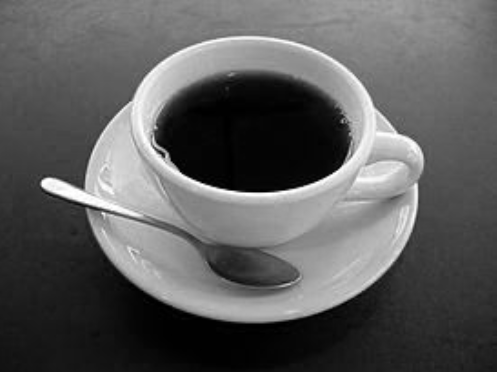
\includegraphics[width=0.33\textwidth]{images/coffee-identity}
      \label{sub:conv:filter:original}
      }
     \subfloat[Filtre contour]{
      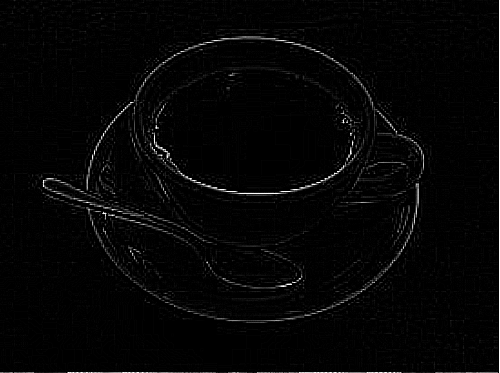
\includegraphics[width=0.33\textwidth]{images/coffee-outline}
      \label{sub:conv:filter:outline}
      }
      \\
      	\subfloat[Filtre de netteté]{
      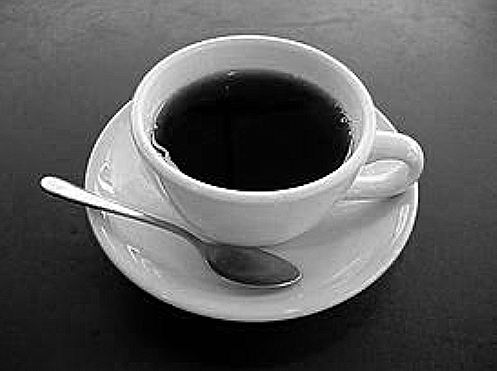
\includegraphics[width=0.33\textwidth]{images/coffee-sharpen}
      \label{sub:conv:filter:sharpen}
      }
     \subfloat[Filtre relief]{
      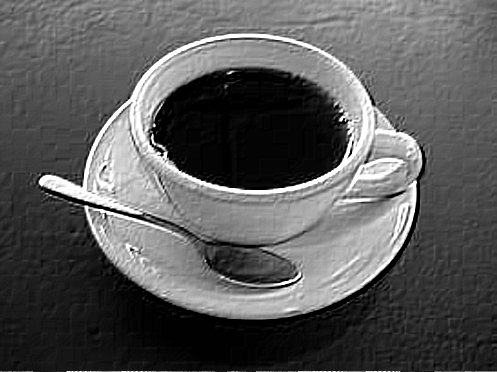
\includegraphics[width=0.33\textwidth]{images/coffee-emboss}
      \label{sub:conv:filter:emboss}
      }
\caption{Différentes filtres de convolution appliquée à une image.}
\label{fig:conv:filter}
\end{figure}

\begin{figure}[H]
\centering
\begin{tikzpicture}
	\matrix (mtr) [matrix of nodes,row sep=-\pgflinewidth, nodes={draw,  minimum size=5.7mm, anchor=center}]
	{
		12 & 46  & 05 & 94 & 25 & 00 & 87\\
		05 & 13  & 01 & 20 & 25 & 00 & 37\\
		72 & 25  & |[fill=red!30]| 88 & |[fill=red!30]| 21 & |[fill=red!30]| 25 & 00 & 99\\
		21 & 74  & |[fill=red!30]| 68 & |[fill=red!30]| 14 & |[fill=red!30]| 15 & 00 & 61\\
		48 & 97  & |[fill=red!30]| 35 & |[fill=red!30]| 52 & |[fill=red!30]| 10 & 00 & 42\\
		11 & 29  & 57 & 00 & 75 & 00 & 12\\
		17 & 01  & 78 & 00 & 50 & 00 & 12\\
		16 & 54  & 00 & 00 & 25 & 00 & 11\\
	};

	\draw[very thick, red] (mtr-3-3.north west) rectangle (mtr-5-5.south east);

	\node [below= of mtr-8-4.south] (lm) {$\bf I$};
	\node[right = 0.2em of mtr] (str) {$* \frac{1}{9}$};

	\matrix (K) [right=0.2em of str,matrix of nodes,row sep=-\pgflinewidth, nodes={draw, fill=blue!30,  minimum size=5.7mm, anchor=center}]
	{
		1 & 1 & 1 \\
		1 & 1 & 1 \\
		1 & 1 & 1 \\
	};
	\node [below = of K-3-2.south] (lk) {$\bf K$};

	\node [right = 0.2em of K] (eq) {$=$};

	\matrix (ret) [right=0.2em of eq,matrix of nodes,row sep=-\pgflinewidth, nodes={draw, minimum size=5.7mm, anchor=center}, nodes in empty cells]
	{
		 &   &  &  &  &  & \\
		 &   &  &  &  &  & \\
		 &   &  &  &  &  & \\
		 &   &  & |[fill=green!30]| 51 &  &  & \\
		 &   &  &  &  &  & \\
		 &   &  &  &  &  & \\
		 &   &  &  &  &  & \\
		 &   &  &  &  &  & \\
	};
	\node [below = of ret-8-4.south] (lim) {${\bf I_{i,j}} * {\bf K}$};

	\draw[very thick, green] (ret-4-4.north west) rectangle (ret-4-4.south east);

	\draw[densely dotted, blue, thick] (mtr-3-3.north west) -- (K-1-1.north west);
	\draw[densely dotted, blue, thick] (mtr-5-3.south west) -- (K-3-1.south west);
	\draw[densely dotted, blue, thick] (mtr-3-5.north east) -- (K-1-3.north east);
	\draw[densely dotted, blue, thick] (mtr-5-5.south east) -- (K-3-3.south east);

	\draw[densely dotted, green, thick] (ret-4-4.north west) -- (K-1-1.north west);
	\draw[densely dotted, green, thick] (ret-4-4.south west) -- (K-3-1.south west);
	\draw[densely dotted, green, thick] (ret-4-4.north east) -- (K-1-3.north east);
	\draw[densely dotted, green, thick] (ret-4-4.south east) -- (K-3-3.south east);

	\draw[very thick, blue] (K-1-1.north west) rectangle (K-3-3.south east);

	\node[anchor=south east, inner sep=0.01em, blue] at (mtr-3-3.south east) (xx) {\scalebox{.5}{$\times 1$}};
	\node[anchor=south east, inner sep=0.01em, blue] at (mtr-3-4.south east) (xx) {\scalebox{.5}{$\times 1$}};
	\node[anchor=south east, inner sep=0.01em, blue] at (mtr-3-5.south east) (xx) {\scalebox{.5}{$\times 1$}};
	\node[anchor=south east, inner sep=0.01em, blue] at (mtr-4-3.south east) (xx) {\scalebox{.5}{$\times 1$}};
	\node[anchor=south east, inner sep=0.01em, blue] at (mtr-4-4.south east) (xx) {\scalebox{.5}{$\times 1$}};
	\node[anchor=south east, inner sep=0.01em, blue] at (mtr-4-5.south east) (xx) {\scalebox{.5}{$\times 1$}};
	\node[anchor=south east, inner sep=0.01em, blue] at (mtr-5-3.south east) (xx) {\scalebox{.5}{$\times 1$}};
	\node[anchor=south east, inner sep=0.01em, blue] at (mtr-5-4.south east) (xx) {\scalebox{.5}{$\times 1$}};
	\node[anchor=south east, inner sep=0.01em, blue] at (mtr-5-5.south east) (xx) {\scalebox{.5}{$\times 1$}};
\end{tikzpicture}
\caption{Convolution d'une matrice (image) (I) par un filtre (K)}
\label{fig:conv:image}
\end{figure}

Étant donné que l'image résultat est une nouvelle image et que le calcul de chaque nouveau pixel de cette image est indépendant des nouveaux pixels voisins, cette opération mathématique est hautement parallélisable et donc fortement prône a l'optimisation et au calcul sur carte graphique.

% Parler de CUDA OpenGL OpenCL CPU
% Parler de convolution érosion
% Benchmark sur un seul PC
% Parler algorithme de detection de gommette

% apres résultat parler de la convolution mega optimisée : avantage et contrainte (convolution en deux temps)

\section{Matériel}
% Benchmark caméra
% Benchmark PC 
% Encoding H264 flux video etc

\section{Nectar - Architecture micro services}
% Schéma dans téléphone a refaire 